\subsubsection*{TSDF Rekonstruktion}

\citet{Klingensmith_2015_7924} erwähnen, dass ihr Verfahren Chisel zunächst als proprietäre Umsetzung im Project Tango Constructor\footnote{Project Tango Constructor - https://goo.gl/8HdTnY (27.02.16)}, Googles Demo Anwendung zur räumlichen Rekonstruktion, umgesetzt wurde. Zu Ihrer Publikation haben sie jedoch zusätzlich eine Open-Source ROS basiertes Modul zur Verfügung gestellt. Diese Bibliothek mit dem Namen OpenChisel\footnote{OpenChisel - Chisel chunked TSDF library - https://goo.gl/nla8hy (27.02.16)} wurde für den Prototypen auf das Android NDK portiert. Dafür wurden einige Module des C++11 Standards, wie zum Beispiel \enquote{st::shared\_ptr}, die zum derzeitigen Kenntnisstand vom Android NDK nicht unterstützt oder anders Umgesetzt werden, auf die Boost\footnote{Boost C++ Libraray - http://www.boost.org/ (27.02.16)} Implementationen abgeändert. Neben der Boost Bibliothek nutzt OpenChisel auch die Eigen Bibliothek für Primitiven und Berechnungen der linearen Algebra.\\

Als Eingabe benötigt OpenChisel neben der Kameraposition und Kameraeigenschaften entweder einer Pointcloud oder ein Tiefenbild. In der Proof of Concept Umsetzung war erkennbar, dass OpenChisel mit der Pointcloud von Project Tango deutlich schlechtere Ergebnisse lieferte, als die Implementation des Constructors von Google. Dadurch, dass die Support Bibliothek von Google seit Februar 2016 eine performante Methode\footnote{TangoSupport\_upsampleImageNearestNeighbor - https://goo.gl/mchIie (27.02.16)} anbietet, um aus einer Punktewolke eine DepthMap mit einer Auflösung von \(320x180\) Pixel zu generieren, wird nun ein Tiefenbild für OpenChisel verwendet. Die resultierenden Ergebnisse kommen dadurch der Constructor Implementation deutlich näher. Abbildung \ref{fig:chisel-demo} zeigt eine exemplarische Rekonstruktion einer Pointcloud links mit dem resultierenden Tiefenbild rechts.

\begin{figure}[h]
  \centering
	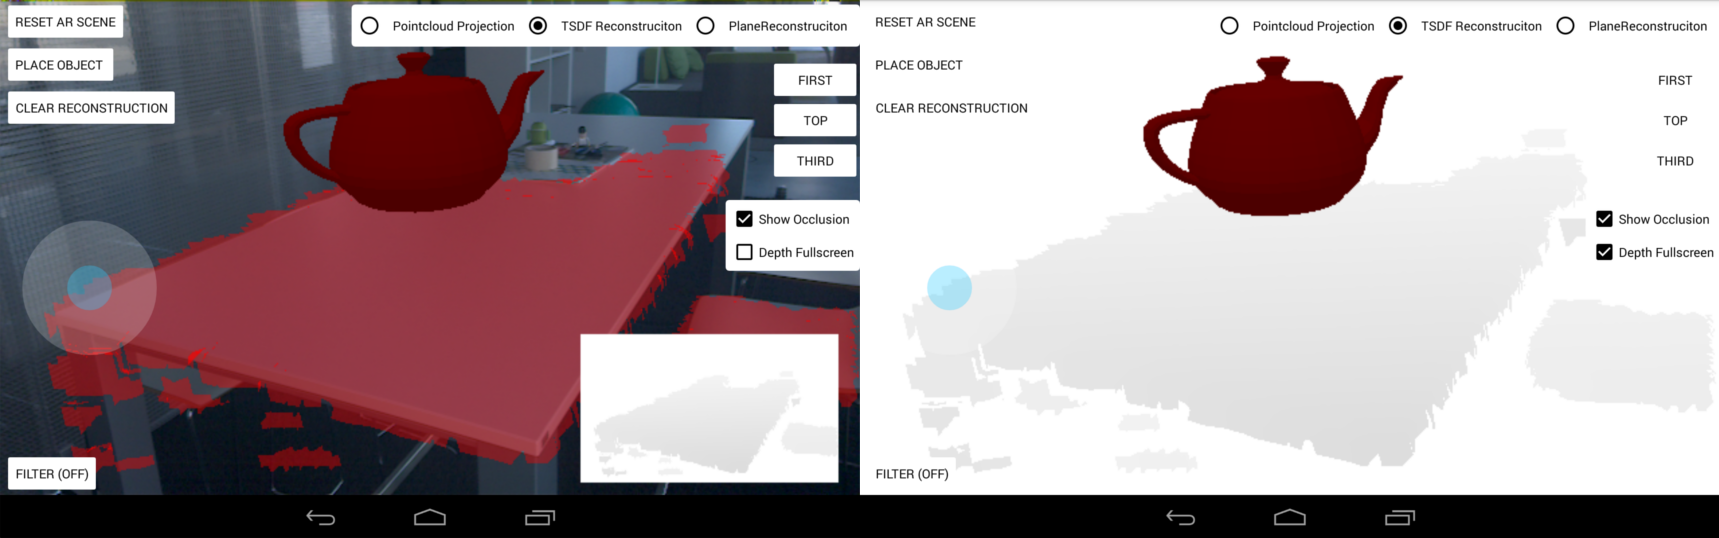
\includegraphics[width=1.0\textwidth]{content/images/implementation/chisel-demo.png} 
  \caption{OpenChisel Rekonstruktion Prototyp. Links optionale Projektion auf der Bildebene. Rechts das resultierende Tiefenbild.}
  \label{fig:chisel-demo}
\end{figure}
